% Template for PLoS
% Version 3.5 March 2018
%
% % % % % % % % % % % % % % % % % % % % % %
%
% -- IMPORTANT NOTE
%
% This template contains comments intended
% to minimize problems and delays during our production
% process. Please follow the template instructions
% whenever possible.
%
% % % % % % % % % % % % % % % % % % % % % % %
%
% Once your paper is accepted for publication,
% PLEASE REMOVE ALL TRACKED CHANGES in this file
% and leave only the final text of your manuscript.
% PLOS recommends the use of latexdiff to track changes during review, as this will help to maintain a clean tex file.
% Visit https://www.ctan.org/pkg/latexdiff?lang=en for info or contact us at latex@plos.org.
%
%
% There are no restrictions on package use within the LaTeX files except that
% no packages listed in the template may be deleted.
%
% Please do not include colors or graphics in the text.
%
% The manuscript LaTeX source should be contained within a single file (do not use \input, \externaldocument, or similar commands).
%
% % % % % % % % % % % % % % % % % % % % % % %
%
% -- FIGURES AND TABLES
%
% Please include tables/figure captions directly after the paragraph where they are first cited in the text.
%
% DO NOT INCLUDE GRAPHICS IN YOUR MANUSCRIPT
% - Figures should be uploaded separately from your manuscript file.
% - Figures generated using LaTeX should be extracted and removed from the PDF before submission.
% - Figures containing multiple panels/subfigures must be combined into one image file before submission.
% For figure citations, please use "Fig" instead of "Figure".
% See http://journals.plos.org/plosone/s/figures for PLOS figure guidelines.
%
% Tables should be cell-based and may not contain:
% - spacing/line breaks within cells to alter layout or alignment
% - do not nest tabular environments (no tabular environments within tabular environments)
% - no graphics or colored text (cell background color/shading OK)
% See http://journals.plos.org/plosone/s/tables for table guidelines.
%
% For tables that exceed the width of the text column, use the adjustwidth environment as illustrated in the example table in text below.
%
% % % % % % % % % % % % % % % % % % % % % % % %
%
% -- EQUATIONS, MATH SYMBOLS, SUBSCRIPTS, AND SUPERSCRIPTS
%
% IMPORTANT
% Below are a few tips to help format your equations and other special characters according to our specifications. For more tips to help reduce the possibility of formatting errors during conversion, please see our LaTeX guidelines at http://journals.plos.org/plosone/s/latex
%
% For inline equations, please be sure to include all portions of an equation in the math environment.
%
% Do not include text that is not math in the math environment.
%
% Please add line breaks to long display equations when possible in order to fit size of the column.
%
% For inline equations, please do not include punctuation (commas, etc) within the math environment unless this is part of the equation.
%
% When adding superscript or subscripts outside of brackets/braces, please group using {}.
%
% Do not use \cal for caligraphic font.  Instead, use \mathcal{}
%
% % % % % % % % % % % % % % % % % % % % % % % %
%
% Please contact latex@plos.org with any questions.
%
% % % % % % % % % % % % % % % % % % % % % % % %

\documentclass[10pt,letterpaper]{article}
\usepackage[top=0.85in,left=2.75in,footskip=0.75in]{geometry}

% amsmath and amssymb packages, useful for mathematical formulas and symbols
\usepackage{amsmath,amssymb}

% Use adjustwidth environment to exceed column width (see example table in text)
\usepackage{changepage}

% Use Unicode characters when possible
\usepackage[utf8x]{inputenc}

% textcomp package and marvosym package for additional characters
\usepackage{textcomp,marvosym}

% cite package, to clean up citations in the main text. Do not remove.
% \usepackage{cite}

% Use nameref to cite supporting information files (see Supporting Information section for more info)
\usepackage{nameref,hyperref}

% line numbers
\usepackage[right]{lineno}

% ligatures disabled
\usepackage{microtype}
\DisableLigatures[f]{encoding = *, family = * }

% color can be used to apply background shading to table cells only
\usepackage[table]{xcolor}

% array package and thick rules for tables
\usepackage{array}

% create "+" rule type for thick vertical lines
\newcolumntype{+}{!{\vrule width 2pt}}

% create \thickcline for thick horizontal lines of variable length
\newlength\savedwidth
\newcommand\thickcline[1]{%
  \noalign{\global\savedwidth\arrayrulewidth\global\arrayrulewidth 2pt}%
  \cline{#1}%
  \noalign{\vskip\arrayrulewidth}%
  \noalign{\global\arrayrulewidth\savedwidth}%
}

% \thickhline command for thick horizontal lines that span the table
\newcommand\thickhline{\noalign{\global\savedwidth\arrayrulewidth\global\arrayrulewidth 2pt}%
\hline
\noalign{\global\arrayrulewidth\savedwidth}}


% Remove comment for double spacing
%\usepackage{setspace}
%\doublespacing

% Text layout
\raggedright
\setlength{\parindent}{0.5cm}
\textwidth 5.25in
\textheight 8.75in

% Bold the 'Figure #' in the caption and separate it from the title/caption with a period
% Captions will be left justified
\usepackage[aboveskip=1pt,labelfont=bf,labelsep=period,justification=raggedright,singlelinecheck=off]{caption}
\renewcommand{\figurename}{Fig}

% Use the PLoS provided BiBTeX style
% \bibliographystyle{plos2015}

% Remove brackets from numbering in List of References
\makeatletter
\renewcommand{\@biblabel}[1]{\quad#1.}
\makeatother



% Header and Footer with logo
\usepackage{lastpage,fancyhdr,graphicx}
\usepackage{epstopdf}
%\pagestyle{myheadings}
\pagestyle{fancy}
\fancyhf{}
%\setlength{\headheight}{27.023pt}
%\lhead{
\includegraphics[width=2.0in]{PLOS-submission.eps}}
\rfoot{\thepage/\pageref{LastPage}}
\renewcommand{\headrulewidth}{0pt}
\renewcommand{\footrule}{\hrule height 2pt \vspace{2mm}}
\fancyheadoffset[L]{2.25in}
\fancyfootoffset[L]{2.25in}
\lfoot{\today}

%% Include all macros below

\newcommand{\lorem}{{\bf LOREM}}
\newcommand{\ipsum}{{\bf IPSUM}}


% Pandoc citation processing

\usepackage{float} \floatplacement{figure}{H} \usepackage{float} \floatplacement{figure}{H} \newcommand{\beginsupplement}{\setcounter{table}{0} \renewcommand{\thetable}{S\arabic{table}} \setcounter{figure}{0} \renewcommand{\thefigure}{S\arabic{figure}}}
\usepackage{booktabs}
\usepackage{longtable}
\usepackage{array}
\usepackage{multirow}
\usepackage{wrapfig}
\usepackage{float}
\usepackage{colortbl}
\usepackage{pdflscape}
\usepackage{tabu}
\usepackage{threeparttable}
\usepackage{threeparttablex}
\usepackage[normalem]{ulem}
\usepackage{makecell}
\usepackage{xcolor}



\usepackage{forarray}
\usepackage{xstring}
\newcommand{\getIndex}[2]{
  \ForEach{,}{\IfEq{#1}{\thislevelitem}{\number\thislevelcount\ExitForEach}{}}{#2}
}

\setcounter{secnumdepth}{0}

\newcommand{\getAff}[1]{
  \getIndex{#1}{}
}

\providecommand{\tightlist}{%
  \setlength{\itemsep}{0pt}\setlength{\parskip}{0pt}}

\begin{document}
\vspace*{0.2in}

% Title must be 250 characters or less.
\begin{flushleft}
{\Large
\textbf\newline{Short-term forecasting of total number of confirmed COVID-19 cases in
South Africa: A Bayesian temporal modelling approach} % Please use "sentence case" for title and headings (capitalize only the first word in a title (or heading), the first word in a subtitle (or subheading), and any proper nouns).
}
\newline
% Insert author names, affiliations and corresponding author email (do not include titles, positions, or degrees).
\\
Belay Birlie Yimer\textsuperscript{\getAff{Arthritis Research UK Centre for Epidemiology, Division of
Musculoskeletal and Dermatological Sciences, The University of
Manchester, Manchester;}, \getAff{Interuniversity Institute for Biostatistics and statistical
Bioinformatics (I-BioStat), Hasselt University, Diepenbeek, Belgium.}},
Ziv Shkedy\textsuperscript{\getAff{Interuniversity Institute for Biostatistics and statistical
Bioinformatics (I-BioStat), Hasselt University, Diepenbeek, Belgium.}}\\
\bigskip
\bigskip
\end{flushleft}
% Please keep the abstract below 300 words
\section*{Abstract}
To be updated.

% Please keep the Author Summary between 150 and 200 words
% Use first person. PLOS ONE authors please skip this step.
% Author Summary not valid for PLOS ONE submissions.
\section*{Author summary}
To be updated.

\linenumbers

% Use "Eq" instead of "Equation" for equation citations.
\hypertarget{introduction}{%
\section{Introduction}\label{introduction}}
Coronaviruses (COVID-19) is an infectious disease that may cause respiratory infections ranging from the common cold to more severe diseases. The novel COVID-19 outbreak was first detected in December 2019 in Wuhan, China. The outbreak later spread to every province of mainland China and 188 other countries, with more than 118 million confirmed cases and more than 2.63 million deaths as of March 8, 2021 [REF]. The first COVID-19 case was reported in South Africa
on 5 March 2020 [REF]. As of March 8, 2021, the number of confirmed COVID-19 cases in Africa represents around 3\% of the infection worldwide. South Africa had the highest burden of COVID-19 cases in the African region, with 1.5 million reported cases and 50,678 confirmed COVID-19 related deaths[REF].

During this period, countries, including South Africa, have adopted various measures to control the virus's spread, including border closure, mandatory use of fabric masks, contact tracing, and stay-at-home measures. Due to the uncertainties about the disease and the need to make informed policy decisions, modelling has taken centre stage in supporting critical policy discussions surrounding COVID-19. COVID-19 modelling studies generally follow one of two general approaches—the phenomenological and mechanistic models. Phenomenological models are statistical models that use generic strategies such as regression to provide quantitative projections that policymakers may need to allocate resources or plan interventions in the short term. On the other hand, mechanistic models use parameters and functional forms to represent our knowledge and assumptions on transmission, disease, and immunity to produce a long-term forecast. 

Several authors implemented phenomenological and mechanistic models to describe the early course of COVID-19 in South Africa and produce short-term and long-term forecasts using the data from the early phase of the epidemic{[}1{]}. In this paper we present (1) South Africa's one year COVID trajectory and (2) fit a series of temporal models to produce short term predictions of the number of reported cases expected for a period of 10 days ahead. 
%Building on popular temporal models, this part of the thesis aims to develop statistical approaches to characterize the course of the COVID-19 outbreak and produce short term forecasts using daily reports of tests and confirmed COVID-19 cases. 


\hypertarget{methods}{%
\section{Methods}\label{methods}}

\hypertarget{data}{%
\subsection{Data}\label{data}}

We downloaded data from Coronavirus COVID-19 (2019-nCoV) Data Repository
for South Africa maintained by Data Science for Social Impact research
group at the University of Pretoria (https://github.com/dsfsi/covid19za). The data repository
captures the daily number of new cases, number of tests, number of
deaths and recoveries. Our primary outcome of interest was the daily
number of newly diagnosed COVID-19 cases and the unit of time used in
modelling was a day. We used the daily case reports from March 12, 2020,
until February 27, 2021, in our analysis.

\hypertarget{statistical-analysis}{%
\subsection{Statistical analysis}\label{statistical-analysis}}

We considered four widely used temporal models to study the evolution of the number of daily COVID-19 cases. We let \(Y(t)\) denote the daily
number of newly diagnosed COVID-19 cases at time \(t\) and \(\mu(t)\)
represent the expected number of cases at time \(t\). We considered a
Negative binomial distribution for \(Y(t)\) to account for possible
overdispersion. That is, \(Y(t) \sim NB(\mu(t), \delta)\), where
\(\delta\) is the overdispersion parameter. We considered four temporal
models to capture the trend over time: a random walk of order one (\(RW(2)\)), a random walk of order (\(RW(2)\)), an autoregressive model of order one (\(AR(1)\)), and an autoregressive model of order two (\(AR(2)\))
{[}2{]} which are presented in Table \ref{tab:Models}. 

%We also considered a \(RW(1)\) model, but the model overfits thedata (See the supplementary appendix). Similarly, we considered an \(AR\)model order \(p=2\) but the result is similar to \(AR1\) model and weprefer the simpler \(AR1\) model.The \(AR(1)\) model {[}1{]} is given by,
%\[
%\begin{aligned}
% Y(t) &\sim NB(\mu(t), \delta) \ \ t=1, \dots, n,\\
% log(\mu(t)) &= \alpha+u_t, \\
% u_1 &\sim N(0, \tau_u(1-\rho^2)^{-1}),  \\
%  u_t &=\rho u_{t-1} +\epsilon_t, \ \ t=2, \dots, n,  \\
%  \epsilon_t & \sim N(0, \tau_{\epsilon}),
%\end{aligned}
%\] where, \(\alpha\) is an intercept, \(\rho\) a temporal correlation
%term (with \(|\rho|<1\)) and \(\epsilon_t\) is a Gaussian error term
%with zero mean and precision \(\tau_{\epsilon}\).

%Similarly, the \(RW(2)\) model {[}1{]} is given by, \[
%\begin{aligned}
% Y(t) &\sim NB(\mu(t), \delta) \ \ t=1, \dots, n,\\
% log(\mu(t)) &= \alpha+u_t, \\
% u_t-2u_{t+1}+u_{t+2} &\sim N(0, \tau_u), \ \ t=2, \dots, n,
%\end{aligned}
%\] where \(\alpha\) is the intercept term as before and \(\tau_u\) is
%the precision parameter.
\begin{table}[!h]
	
	\caption{\label{tab:Models}Model formulation for the Bayesian temporal models fitted to COVID-19 outbreak data. Note that $Y(t)$ is the daily number of COVID-19 cases and \(Y(t) \sim NB(\mu(t), \delta)\).}
	\centering
	\begin{tabular}[t]{ccc}
		\hline
		Model& & \\
		\hline
		\(AR(1)\)& & $\begin{aligned}[t]
		log(\mu(t)) &= \alpha+u_t,\\
		u_1 &\sim N(0, \tau_u(1-\rho^2)^{-1}),\\
		u_t &=\rho u_{t-1} +\epsilon_t, \ \ t=2, \dots, n,\\
		\epsilon_t & \sim N(0, \tau_{\epsilon}),
		\end{aligned}$\\
		& & \\
		\(AR(2)\)& &$\begin{aligned}[t]
		log(\mu(t)) &= \alpha+u_t,\\
		u_t &=\rho_1 u_{t-1}+\rho_2 u_{t-2} +\epsilon_t, \ \ t=2, \dots, n,\\
		\epsilon_t & \sim N(0, \tau_{\epsilon}),
		\end{aligned}$\\
		& & \\
		\(RW(1)\)& &  $\begin{aligned}[t]
		log(\mu(t)) &= \alpha+u_t, \\
		u_t-u_{t-1} &\sim N(0, \tau_u), \ \ t=2, \dots, n,
		\end{aligned}$\\
		& & \\
		\(RW(2)\)& &  $\begin{aligned}[t]
		log(\mu(t)) &= \alpha+u_t, \\
		u_t-2u_{t+1}+u_{t+2} &\sim N(0, \tau_u), \ \ t=2, \dots, n,
		\end{aligned}$\\
		\hline
	\end{tabular}
\end{table}

Each models were fitted within the Bayesian framework using
\emph{inla} {[}3{]}. To complete the specification of each models, we
assume the following priors. For both the \(RW(1)\) and \(RW(2)\), we represent the precision parameter of
\(\tau_u\) as \(\theta=log(\tau_u)\) and assume a
\(\Gamma (10,100)\) prior for \(\theta\).  For the \(AR(1)\) model, we denote
\(\theta_1=log(\tau_u(1-\rho^2))\) where \(\Gamma(10,100)\) prior is
specified for \(\theta_1\), and we denote
\(\theta_2=log\frac{1+\rho}{1-\rho}\) and assume a \(N(0, 0.15)\) prior
for \(\theta\). 

The short-term prediction performance of all these models were evaluated using mean absolute error (MAE), mean absolute percentage error (MAPE), and chi-squared value. Additionally, the model fits were evaluated by using Deviance information criteria (DIC) {[}5{]} and Watanabe–Akaike information criterion (WAIC){[}5{]}. The R-codes that we used for our analyses are available at
https://github.com/belayb/COVIDincidenceSA.



\hypertarget{results}{%
\section{Results}\label{results}}

The daily number of reported COVID-19 cases from 12
March 2020 to 27 February 2021 is presented in Figure \ref{fig:daily-cases}. Similar to elsewhere in the world, South
Africa pass through a two-wave pandemic. The pandemic first peak was
on 07 July 2020, where up to 13944 new COVID-19 cases reported, followed
by a second peak in January 2021, where more than 21,000 daily cases
reported. Figure \ref{fig:cummulative} presents the cumulative number of reported
COVID-19 cases and tests performed. To date, 8,838,937 tests have been
conducted, and a total of 1,500,677 cases reported.

\begin{figure}[H]
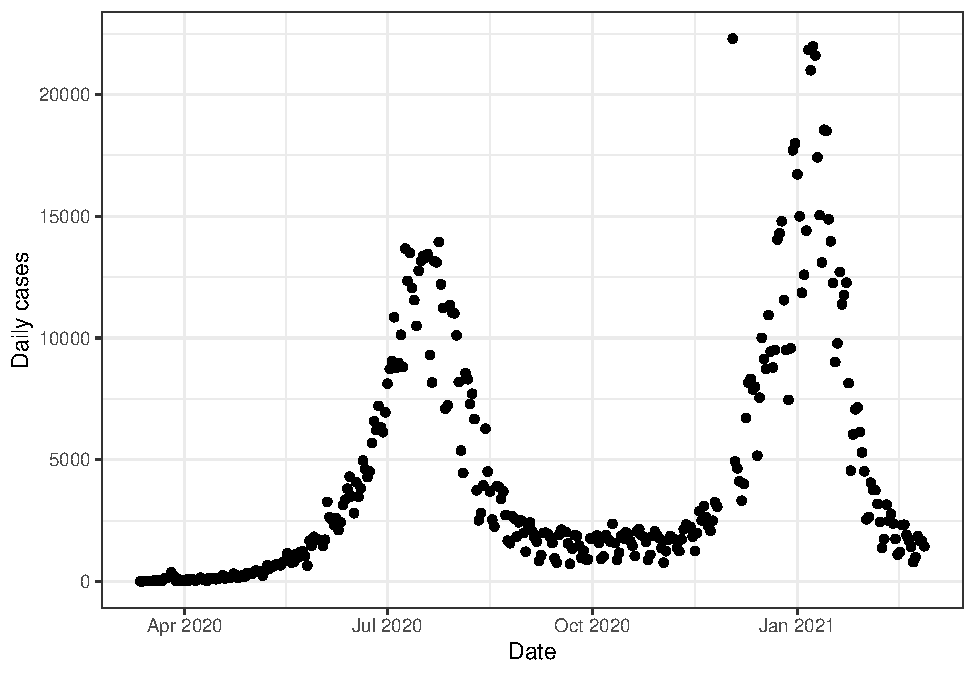
\includegraphics[width=0.99\linewidth]{COVIDincidenceSA_files/figure-latex/daily-cases-1} \caption{Daily number of COVID-19 cases in South Africa from 12/03/2020-27/02/2021.}\label{fig:daily-cases}
\end{figure}

\begin{figure}[H]
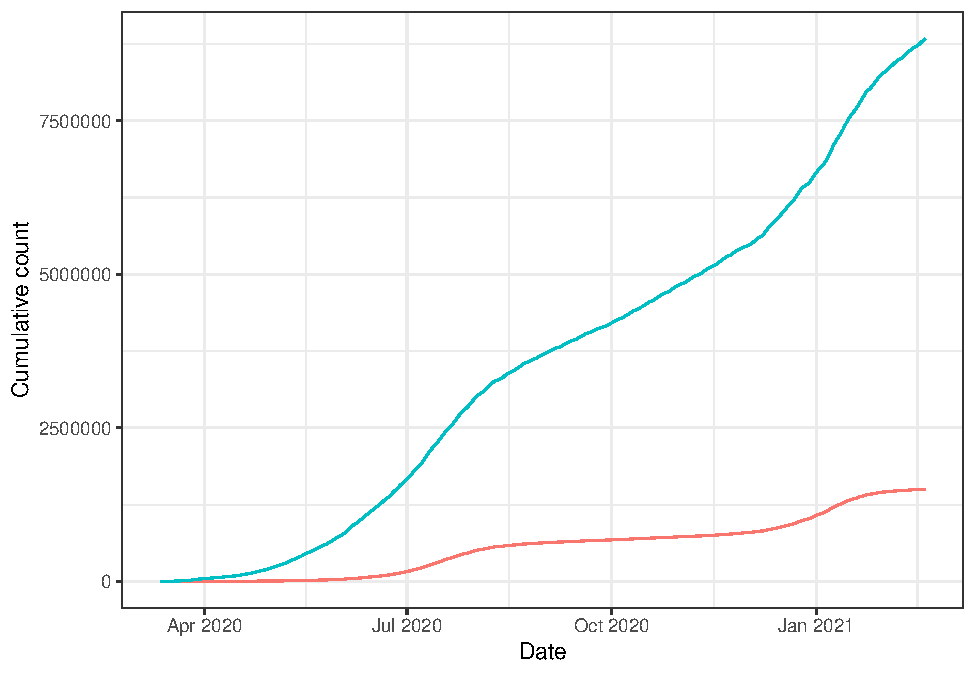
\includegraphics[width=0.99\linewidth]{COVIDincidenceSA_files/figure-latex/cummulative-1} \caption{The cumulative number of COVID-19 cases and cumulative number of tests in South Africa from 12/03/2020-27/02/2021. Red-line denote the number of cases and blue-line denotes the number of tests.}\label{fig:cummulative}
\end{figure}

\hypertarget{short-term-prediction-of-the-total-number-of-reported-covid-19-cases}{%
\subsection{Short-term prediction of the total number of reported
COVID-19
cases}\label{short-term-prediction-of-the-total-number-of-reported-covid-19-cases}}

We fit the four models described in the previous section to the daily
reported new COVID-19 cases. The models were fitted to the data from 12/03/2020-07/02/2021 (estimation period). The parameter estimates for each of the fitted models
are presented in Supplementary Table \ref{tab:parest}. Our main interest to produce a short-term forecast for the number of reported cases.  Figure \ref{fig:ar1fitted} - \ref{fig:rw2fitted} in the supplementary appendix presents the fitted model to the observed data (panel A) and the first-order derivative of the fitted curve for each model. All models considered appear to fit the observed data (within the estimation period) well. Nonetheless, the \(AR(1)\), \(AR(2)\), and \(RW(1)\) tend to overfit the data. 

Figure \ref{fig:10daypred} and Table \ref{tab:10daypred} presents 10-days ahead forecasting of the cumulative COVID-19 cases for each model. The \(AR(1)\), \(AR(2)\), and \(RW(1)\) models performed well for the first three forecasting days and overestimated the cumulative cases from day three onward. The overestimation worsens for these models as we move further from the estimation period. On the other hand, the \(RW(2)\) performed well, showing a consistent prediction performance throughout the forecasting period.  The prediction error (\(observed - predicted\)) for \(RW(2)\) stays between 1932 and 3222 cases, whereas the prediction error linearly increase for the other models. 

Table \ref{tab:Accuracy} presents the accuracy metrics for each model. The mean absolute error, mean absolute percentage error and Chi-square statistic favours \(RW(2)\) as the best model predictive model. On the other hand, DIC and WAIC favours \(RW(1)\) model. This is expected given that the DIC and WAIC evaluate model performance within estimation period. 

\begin{figure}[!h]
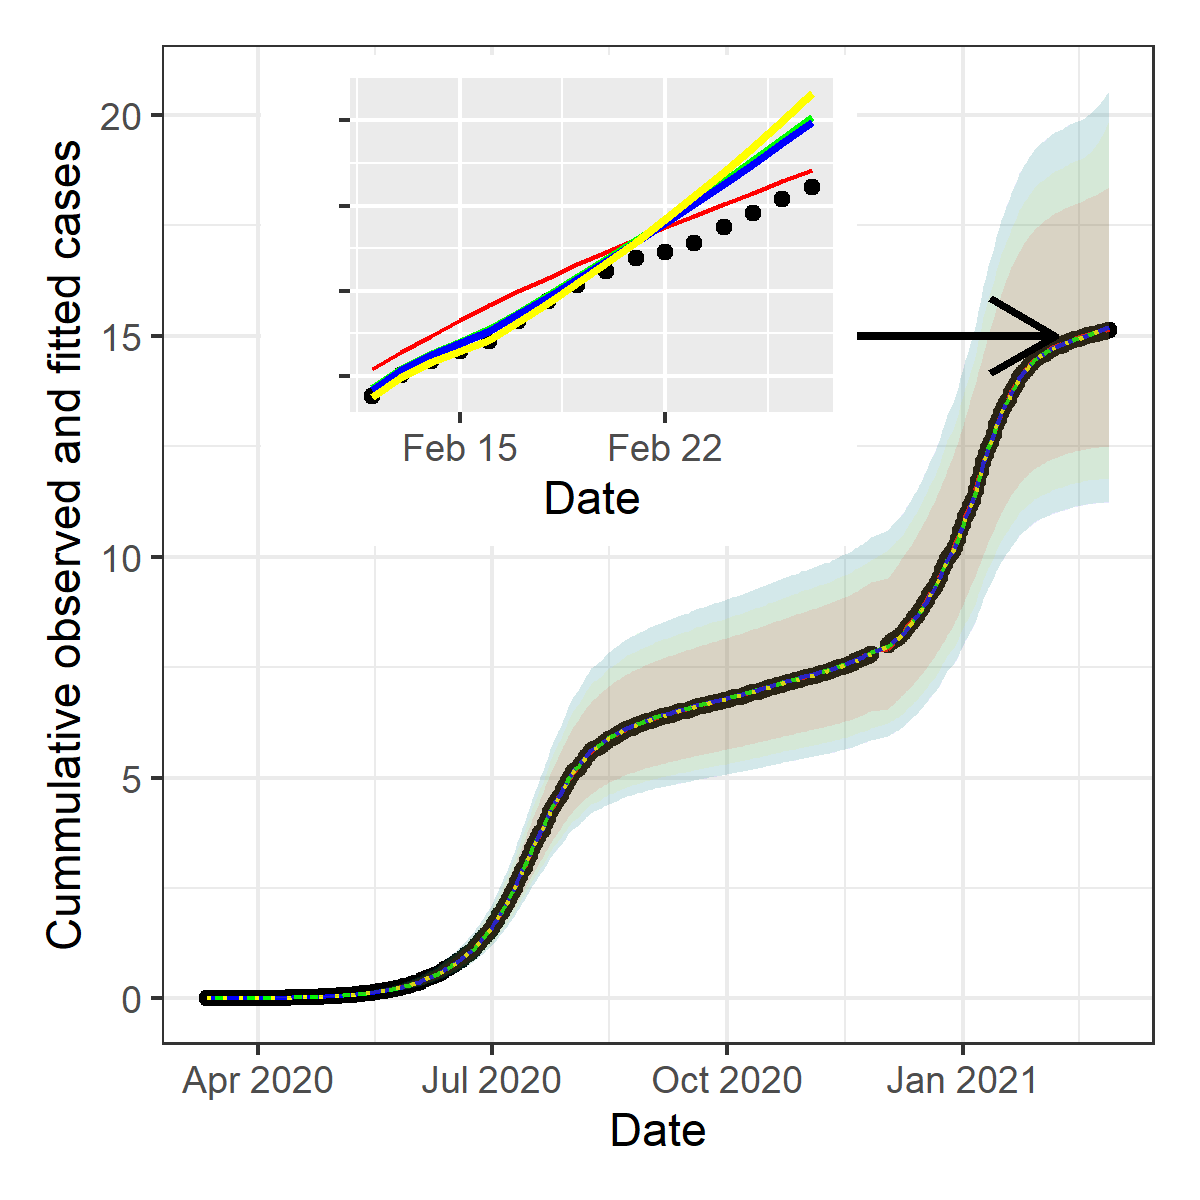
\includegraphics[width=0.99\linewidth]{forcast_cum_all.png} \caption{Ten days a head predicted cumulative COVID-19 cases (per 100, 000) in South Africa under the RW1 (yellow line), RW2 (red line), AR1 (green line), and AR2 (blue line) model. Estimation period 12/03/2020-17/02/2021. The black dots are the observed cumulative cases.The shaded bands are the prediction intervals. }\label{fig:10daypred}
\end{figure}

\begin{table}[!h]

\caption{\label{tab:10daypred}Short-term predictions of total number of reported cases at the national level under the four models. Estimation period 12/03/2020-17/02/2021}
\centering
\resizebox{\textwidth}{!}{\begin{tabular}[t]{l|l|r|r|l|r}
\hline
Model&Date & Total & Prediction & Prediction Interval & Total - Prediction\\
\hline
RW1&2021-02-18 & 1498766 & 1498569 & (1171371.01-1905725.92) & 197.3859\\
&2021-02-19 & 1500677 & 1500866 & (1172282.33-1910642.87) & -188.6823\\
&2021-02-20 & 1502367 & 1503262 & (1173049.22-1916495.57) & -894.6407\\
&2021-02-21 & 1503796 & 1505761 & (1173711.18-1923283.63) & -1964.7423\\
&2021-02-22 & 1504588 & 1508368 & (1174292.27-1931023.86) & -3779.5408\\
&2021-02-23 & 1505586 & 1511087 & (1174808.38-1939743.02) & -5500.8398\\
&2021-02-24 & 1507448 & 1513924 & (1175270.86-1949474.01) & -6475.6849\\
&2021-02-25 & 1509124 & 1516883 & (1175688.37-1960253.97) & -7759.3666\\
&2021-02-26 & 1510778 & 1519971 & (1176067.58-1972123.43) & -9193.4282\\
&2021-02-27 & 1512225 & 1523194 & (1176413.76-1985125.8) & -10968.6766\\
\hline
RW2&2021-02-18 & 1498766 & 1501550 & (1243364.14-1808126.44) & -2784.084\\
&2021-02-19 & 1500677 & 1503091 & (1244303.4-1810572.89) & -2414.449\\
&2021-02-20 & 1502367 & 1504581 & (1245125.49-1813126.02) & -2213.984\\
&2021-02-21 & 1503796 & 1506026 & (1245838.81-1815814.63) & -2229.618\\
&2021-02-22 & 1504588 & 1507432 & (1246452.98-1818667.83) & -2844.351\\
&2021-02-23 & 1505586 & 1508808 & (1246978.01-1821716.68) & -3222.321\\
&2021-02-24 & 1507448 & 1510161 & (1247424.13-1824995.35) & -2712.894\\
&2021-02-25 & 1509124 & 1511498 & (1247800.94-1828542.17) & -2373.747\\
&2021-02-26 & 1510778 & 1512827 & (1248117.46-1832400.55) & -2048.995\\
&2021-02-27 & 1512225 & 1514157 & (1248381.83-1836620.02) & -1932.342\\
\hline
AR1&2021-02-18 & 1498766 & 1499490 & (1118111.85-1994222.05) & -723.8101\\
&2021-02-19 & 1500677 & 1501589 & (1119005.83-1998492.97) & -911.8181\\
&2021-02-20 & 1502367 & 1503742 & (1119771.48-2003403.42) & -1374.5498\\
&2021-02-21 & 1503796 & 1505948 & (1120441.58-2008928.37) & -2152.4467\\
&2021-02-22 & 1504588 & 1508210 & (1121036.44-2015054.48) & -3622.1451\\
&2021-02-23 & 1505586 & 1510527 & (1121570.32-2021775.18) & -4941.3574\\
&2021-02-24 & 1507448 & 1512901 & (1122053.58-2029087.04) & -5452.8340\\
&2021-02-25 & 1509124 & 1515331 & (1122494.04-2036989.06) & -6207.3481\\
&2021-02-26 & 1510778 & 1517820 & (1122897.79-2045481.78) & -7041.6895\\
&2021-02-27 & 1512225 & 1520367 & (1123269.68-2054566.81) & -8141.6604\\
\hline
AR2&2021-02-18 & 1498766 & 1499297 & (1117410.1-1994516.93) & -530.9910\\
&2021-02-19 & 1500677 & 1501378 & (1118308.28-1998709.43) & -701.0323\\
&2021-02-20 & 1502367 & 1503507 & (1119078.99-2003512.61) & -1140.4836\\
&2021-02-21 & 1503796 & 1505686 & (1119754.71-2008896.75) & -1889.5478\\
&2021-02-22 & 1504588 & 1507912 & (1120355.57-2014844.05) & -3324.2951\\
&2021-02-23 & 1505586 & 1510188 & (1120895.7-2021343.34) & -4601.9776\\
&2021-02-24 & 1507448 & 1512513 & (1121385.41-2028386.98) & -5064.8673\\
&2021-02-25 & 1509124 & 1514887 & (1121832.47-2035969.53) & -5763.2504\\
&2021-02-26 & 1510778 & 1517311 & (1122242.95-2044087.07) & -6533.4176\\
&2021-02-27 & 1512225 & 1519786 & (1122621.69-2052736.67) & -7560.6602\\
\hline
\end{tabular}}
\end{table}

\begin{table}[!h]
	
	\caption{\label{tab:Accuracy}Accuracy metrics of forecasting for AR1, AR2, RW1, and RW2 models.}
	\centering
	\resizebox{\textwidth}{!}{\begin{tabular}[t]{lrrrr}
		\hline
		Days ahead point forecasts & \multicolumn{4}{c}{Mean Absolute Error}\\
		\cline{2-5}
		& RW1 & RW2 & AR1 & AR2\\
		\hline
		One day & 567.1704 & 3403.052 & 1100.229 & 975.1169\\
		\hline
		Two day & 1395.0619 & 3048.159 & 1503.359 & 1412.4527\\
		\hline
		Three day & 2309.8792 & 2756.448 & 2273.296 & 2200.8456\\
		\hline
		Four day & 3223.8908 & 2668.973 & 3057.519 & 2971.4183\\
		\hline
		Five day & 4076.6772 & 2722.319 & 3756.599 & 3653.5679\\
		\hline
		Six day & 4677.8180 & 2760.561 & 4178.428 & 4055.0046\\
		\hline
		Seven day & 5121.6867 & 2691.375 & 4415.616 & 4268.1508\\
		\hline
		Eight day & 5897.6715 & 2928.744 & 5036.350 & 4844.4758\\
		\hline
		Nine day & 6041.0341 & 2896.269 & 5119.785 & 4921.4926\\
		\hline
		Ten day & 6218.5109 & 2884.603 & 5229.782 & 5024.2168\\
		\hline
		& \multicolumn{4}{c}{Mean Absolute Percentage Error}\\
		\cline{2-5}\\
		& RW1 & RW2 & AR1 & AR2\\
		\hline\\
		One day & 0.0003807 & 0.0022844 & 0.0007385 & 0.0006546\\
		\hline
		Two day & 0.0009354 & 0.0020427 & 0.0010073 & 0.0009465\\
		\hline
		Three day & 0.0015467 & 0.0018446 & 0.0015218 & 0.0014734\\
		\hline
		Four day & 0.0021564 & 0.0017840 & 0.0020448 & 0.0019873\\
		\hline
		Five day & 0.0027235 & 0.0018176 & 0.0025094 & 0.0024406\\
		\hline
		Six day & 0.0031213 & 0.0018410 & 0.0027877 & 0.0027055\\
		\hline
		Seven day & 0.0034128 & 0.0017925 & 0.0029418 & 0.0028437\\
		\hline
		Eight day & 0.0039270 & 0.0019498 & 0.0033531 & 0.0032256\\
		\hline
		Nine day & 0.0040213 & 0.0019282 & 0.0034079 & 0.0032762\\
		\hline
		Ten day & 0.0041381 & 0.0019203 & 0.0034802 & 0.0033437\\
		\hline
		& \multicolumn{4}{c}{Chi Square}\\
		\cline{2-5}\\
		& RW1 & RW2 & AR1 & AR2\\
		\hline
		One day & 3.526026 & 80.43788 & 10.14578 & 7.642623\\
		\hline
		Two day & 16.552333 & 71.66942 & 22.21648 & 19.346128\\
		\hline
		Three day & 41.883130 & 70.78339 & 46.44967 & 42.301887\\
		\hline
		Four day & 79.235781 & 71.27488 & 79.45425 & 72.947524\\
		\hline
		Five day & 128.010230 & 72.74404 & 119.51466 & 109.013108\\
		\hline
		Six day & 185.934034 & 72.11017 & 162.88745 & 146.770096\\
		\hline
		Seven day & 254.268157 & 71.58625 & 210.31240 & 187.416759\\
		\hline
		Eight day & 293.981286 & 75.31508 & 235.73996 & 209.342520\\
		\hline
		Nine day & 309.899980 & 74.36227 & 242.98123 & 215.549116\\
		\hline
		Ten day & 333.287057 & 74.05306 & 253.91151 & 225.029683\\
		\hline
		\hline\\
		& \multicolumn{4}{c}{Information Criteria}\\
		\hline\\
		DIC & 5059.06 & 5447.40 & 5278.87 & 5284.00\\
		WAIC & 5123.56 & 5460.81 & 5286.90 & 5294.74\\
		\hline\\
	\end{tabular}}
\end{table}


\newpage
\hypertarget{results}{%
\section{Discussion}\label{Discussion}}

Reliable and accurate short-term forecasts of COVID-19 cases are critical to understand the progress of the pandemic in a country and to evaluate the impact of intervention measures in controlling the pandemic. This study modelled COVID-19 cases in South Africa at the national level using publicly available data from 12 March 2020 to 17 February 2021. We have evaluated four widely used temporal models for forecasting confirmed cases of COVID-19 for South Africa. Our study showed that these established temporal models could provide robust and accurate short-term forecasts for a period ten days ahead. The random-walk model of order two was superior to the random-walk of order one and autoregressive models in forecasting performance.  

This study's strength is that the analysis was based on readily accessible, publicly available data that is updated in real-time. The statistical methods applied are relatively simple, implemented using off-the-shelf open-source software, and are not dependent on any assumptions regarding COVID-19 transmission dynamics. 

In summary, we have shown the usefulness of established temporal models to provide short term forecasts of the cumulative COVID-19 cases. Such models could help in decision-making when knowledge regarding factors affecting transmission-dynamics of the disease is limited.  

\newpage
\hypertarget{references}{%
	\section*{References}\label{references}}
\addcontentsline{toc}{section}{References}

\begin{itemize}
	\item[1.] Reddy T, Shkedy Z, van Rensburg CJ, Mwambi H, Debba P, Zuma K, Manda S. Short-term real-time prediction of total number of reported COVID-19 cases and deaths in South Africa: a data driven approach. BMC medical research methodology. 2021 Dec;21(1):1-1.
	
	\item[2.] Gómez-Rubio V. Bayesian inference with INLA. CRC Press; 2020 Feb 20.
	
	\item[3.] Martins TG, Simpson D, Lindgren F, Rue H. Bayesian computing with
	inla: New features. Computational Statistics \& Data Analysis. Elsevier;
	2013;67: 68--83.
	\item[4.] Spiegelhalter DJ, Best NG, Carlin BP, Van der Linde A. The deviance information criterion: 12 years on. Journal of the Royal Statistical Society: Series B: Statistical Methodology. 2014 Jun 1:485-93.
	\item[5.] Watanabe S, Opper M. Asymptotic equivalence of Bayes cross validation and widely applicable information criterion in singular learning theory. Journal of machine learning research. 2010 Dec 1;11(12).
	
\end{itemize}
\nolinenumbers
\newpage
\hypertarget{appendix}{%
\section{Appendix}\label{appendix}}

\setcounter{table}{0} \renewcommand{\thetable}{S\arabic{table}} \setcounter{figure}{0} \renewcommand{\thefigure}{S\arabic{figure}}

\begin{figure}[h]
	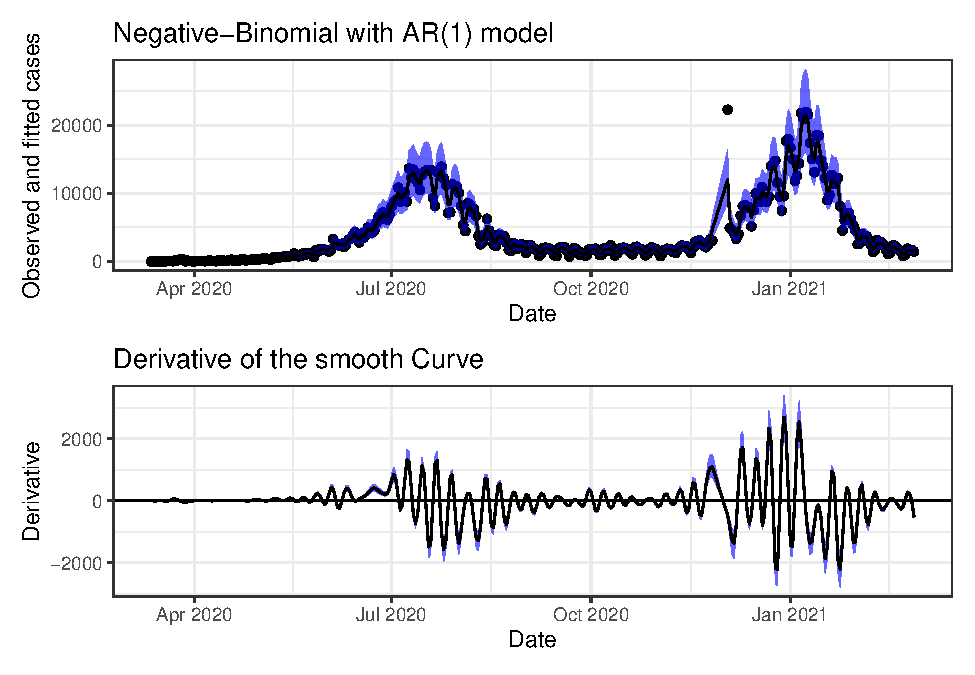
\includegraphics[width=0.99\linewidth]{COVIDincidenceSA_files/figure-latex/unnamed-chunk-6-1} \caption{AR1 model for the daily confirmed COVID-19 cases in South Africa 12/03/2020-27/02/2021.  Panel A-fitted and observed data. The balck dotes are the observed number of daily cases, the black solid line the fitted curve, and the blue shaded area is the 95\% credible interval. Panel B-first-order derivative of the fitted curve along with the 95\% credible interval.}\label{fig:ar1fitted}
\end{figure}

\begin{figure}[h]
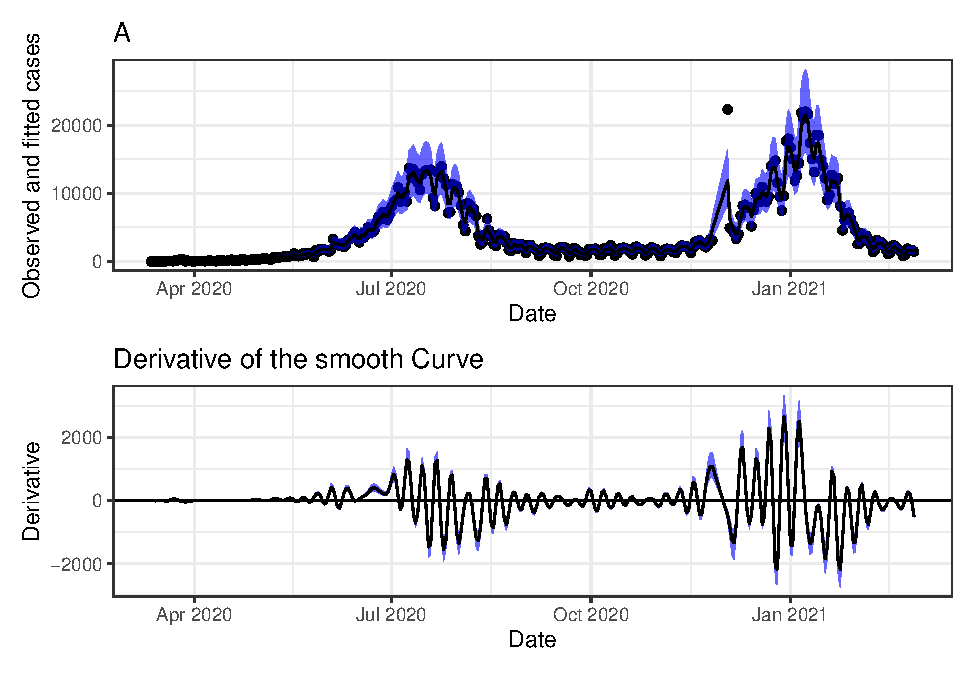
\includegraphics[width=0.99\linewidth]{COVIDincidenceSA_files/figure-latex/unnamed-chunk-13-1} \caption{AR2 model for the daily confirmed COVID-19 cases in South Africa 12/03/2020-27/02/2021.  Panel A-fitted and observed data. The balck dotes are the observed number of daily cases, the black solid line the fitted curve, and the blue shaded area is the 95\% credible interval. Panel B-first-order derivative of the fitted curve along with the 95\% credible interval.}\label{fig:ar2fitted}
\end{figure}

\begin{figure}[h]
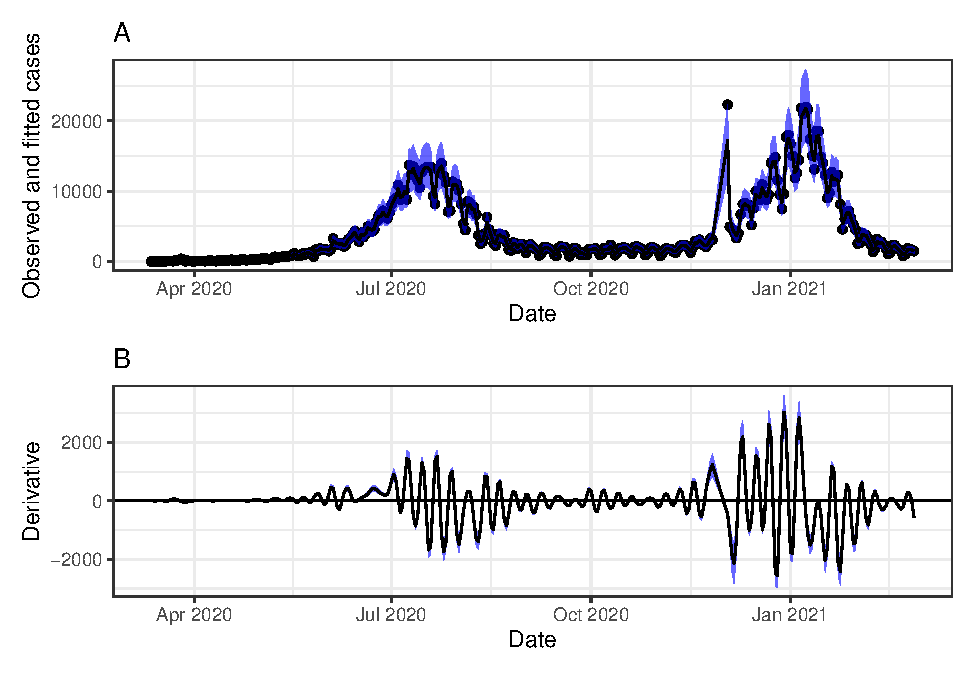
\includegraphics[width=0.99\linewidth]{COVIDincidenceSA_files/figure-latex/unnamed-chunk-14-1} \caption{RW1 model for the daily confirmed COVID-19 cases in South Africa 12/03/2020-27/02/2021.  Panel A-fitted and observed data. The balck dotes are the observed number of daily cases, the black solid line the fitted curve, and the blue shaded area is the 95\% credible interval. Panel B-first-order derivative of the fitted curve along with the 95\% credible interval.}\label{fig:rw1fitted}
\end{figure}

\begin{figure}[h]
	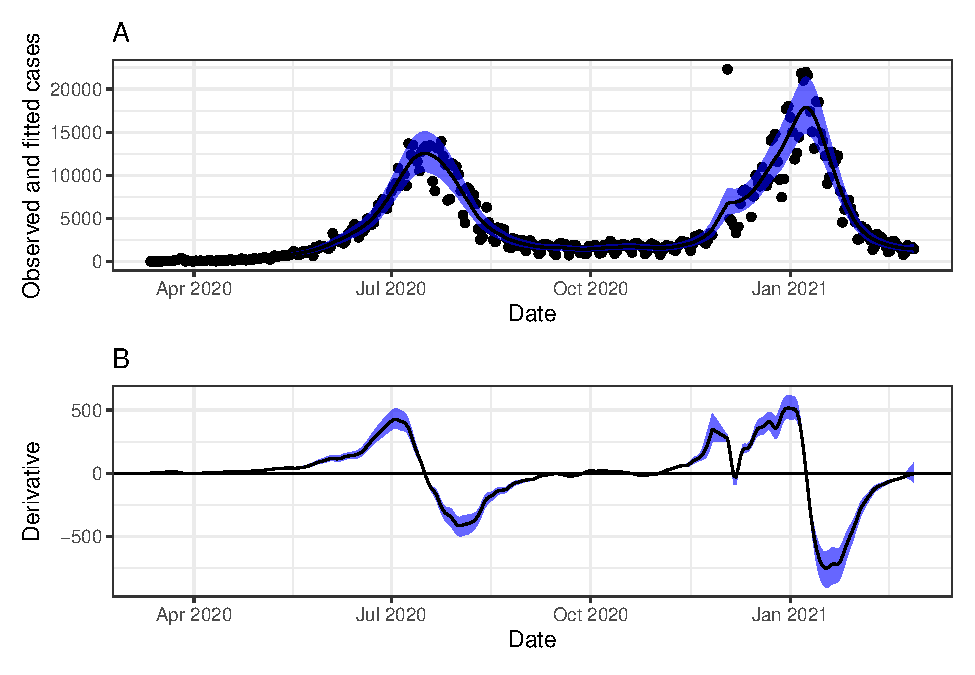
\includegraphics[width=0.95\linewidth]{COVIDincidenceSA_files/figure-latex/unnamed-chunk-7-1} \caption{RW2 model for the daily confirmed COVID-19 cases in South Africa 12/03/2020-27/02/2021.  Panel A-fitted and observed data. The balck dotes are the observed number of daily cases, the black solid line the fitted curve, and the blue shaded area is the 95\% credible interval. Panel B-first-order derivative of the fitted curve along with the 95\% credible interval.}\label{fig:rw2fitted}
\end{figure}

\begin{table}[h]
	
	\caption{\label{tab:parest}Parameter estimates for each model}
	\centering
	\begin{tabular}[t]{l|l|r|r|r|r}
		\hline
		Model& & mean & sd & Lower & upper\\
		\hline
		AR1&(Intercept) & 6.109 & 2.441 & 0.145 & 10.569\\
		&Size & 28.955 & 8.389 & 16.805 & 49.397\\
		&Precision for time & 0.158 & 0.112 & 0.023 & 0.438\\
		&Rho for time & 0.995 & 0.004 & 0.985 & 0.999\\
		\hline
		& &  &  &  & \\
		AR2&(Intercept) & 6.307 & 1.659 & 2.475 & 9.299\\
		&Size & 28.399 & 8.492 & 15.999 & 49.001\\
		&Precision for time & 0.236 & 0.126 & 0.066 & 0.547\\
		&PACF1 for time & 0.992 & 0.005 & 0.980 & 0.998\\
		&PACF2 for time & 0.007 & 0.085 & 0.006 & 0.177\\
		\hline
		& &  &  &  & \\
		RW1 & (Intercept) & 7.565 & 0.001 & 7.564 & 7.587\\
		& Size & 53.685 & 24.186 & 24.47 & 116.45\\
		& Precision for time & 0.231 & 0.044 & 0.15 & 0.23\\
		\hline
		& &  &  &  & \\
		RW2 & (Intercept) & 7.603 & 0.017 & 7.570 & 7.637\\
		& Size & 10.422 & 0.911 & 8.734 & 12.319\\
		& Precision for time & 0.036 & 0.014 & 0.016 & 0.070\\
		\hline
	\end{tabular}
\end{table}

\begin{figure}[h]
	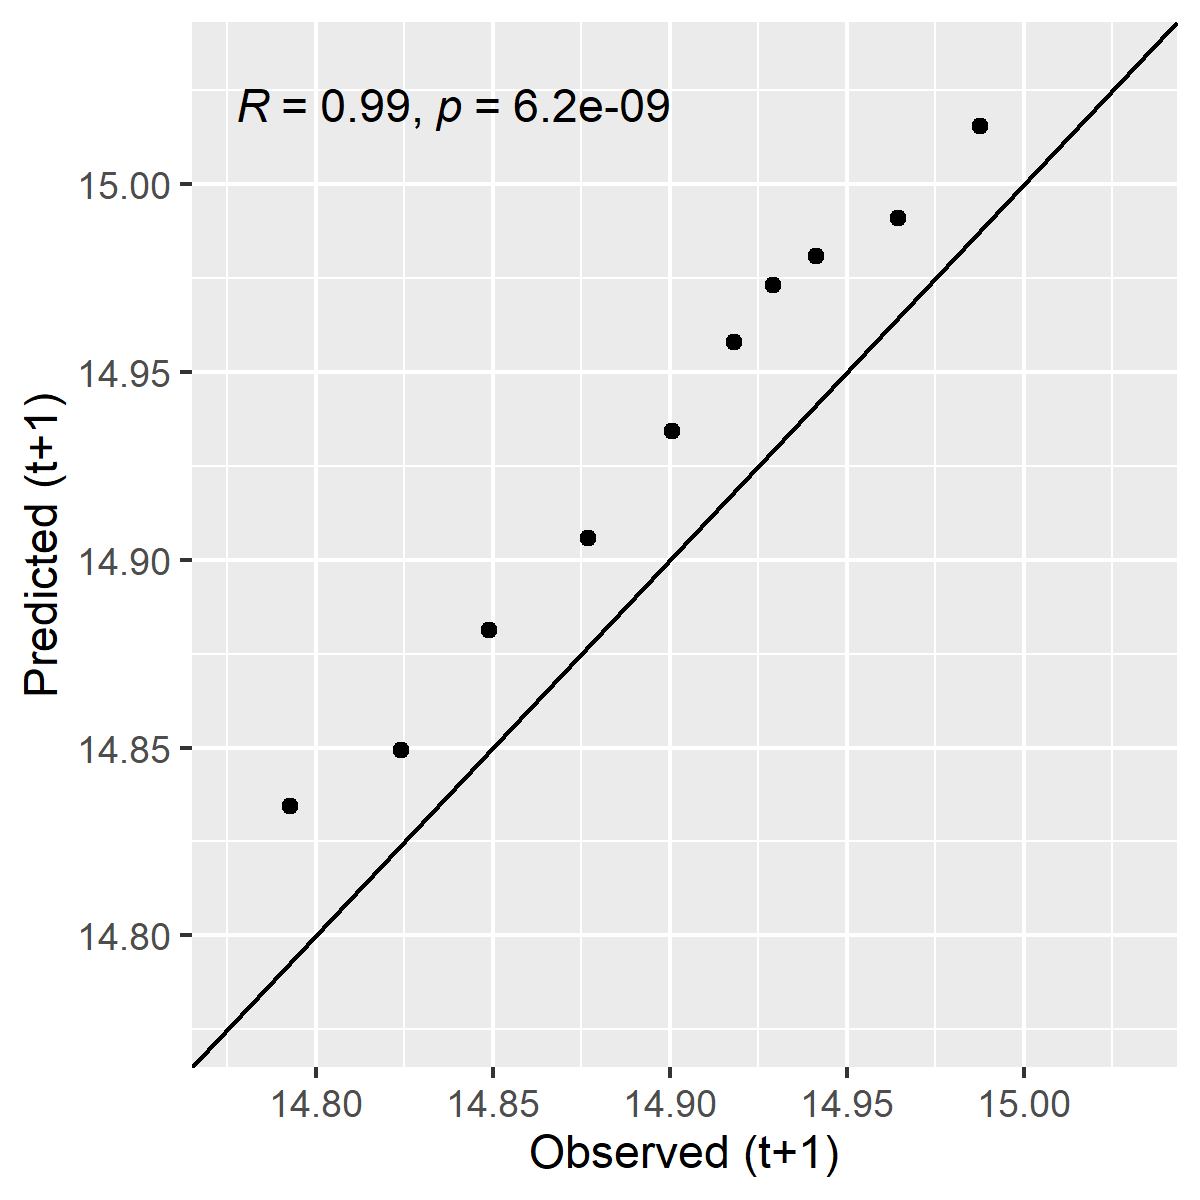
\includegraphics[width=0.3\linewidth]{day1} 
		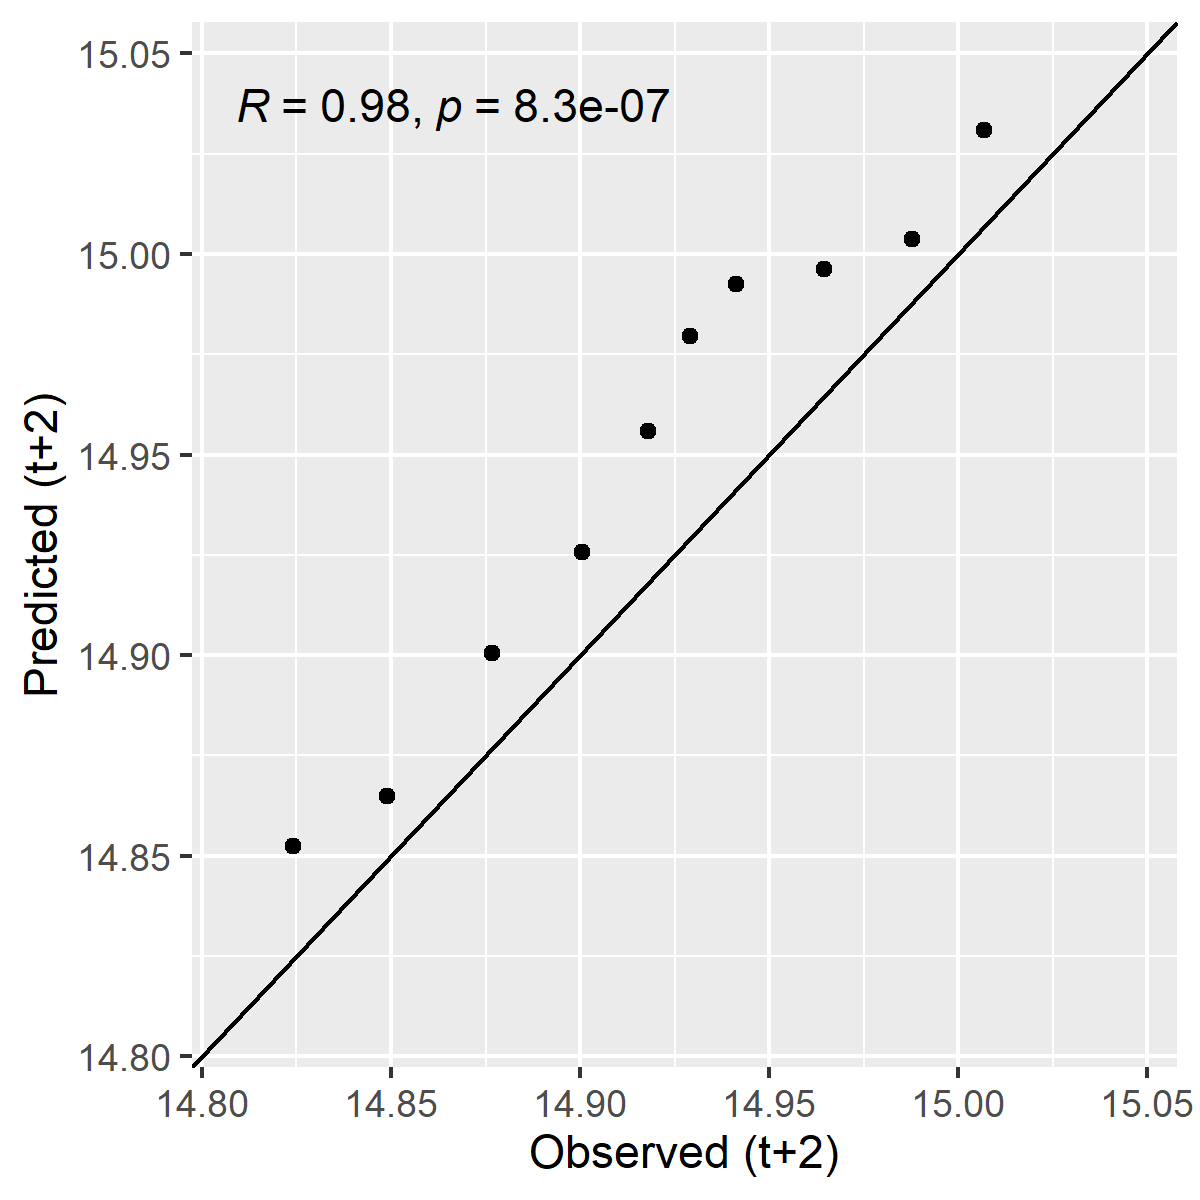
\includegraphics[width=0.3\linewidth]{day2} 
			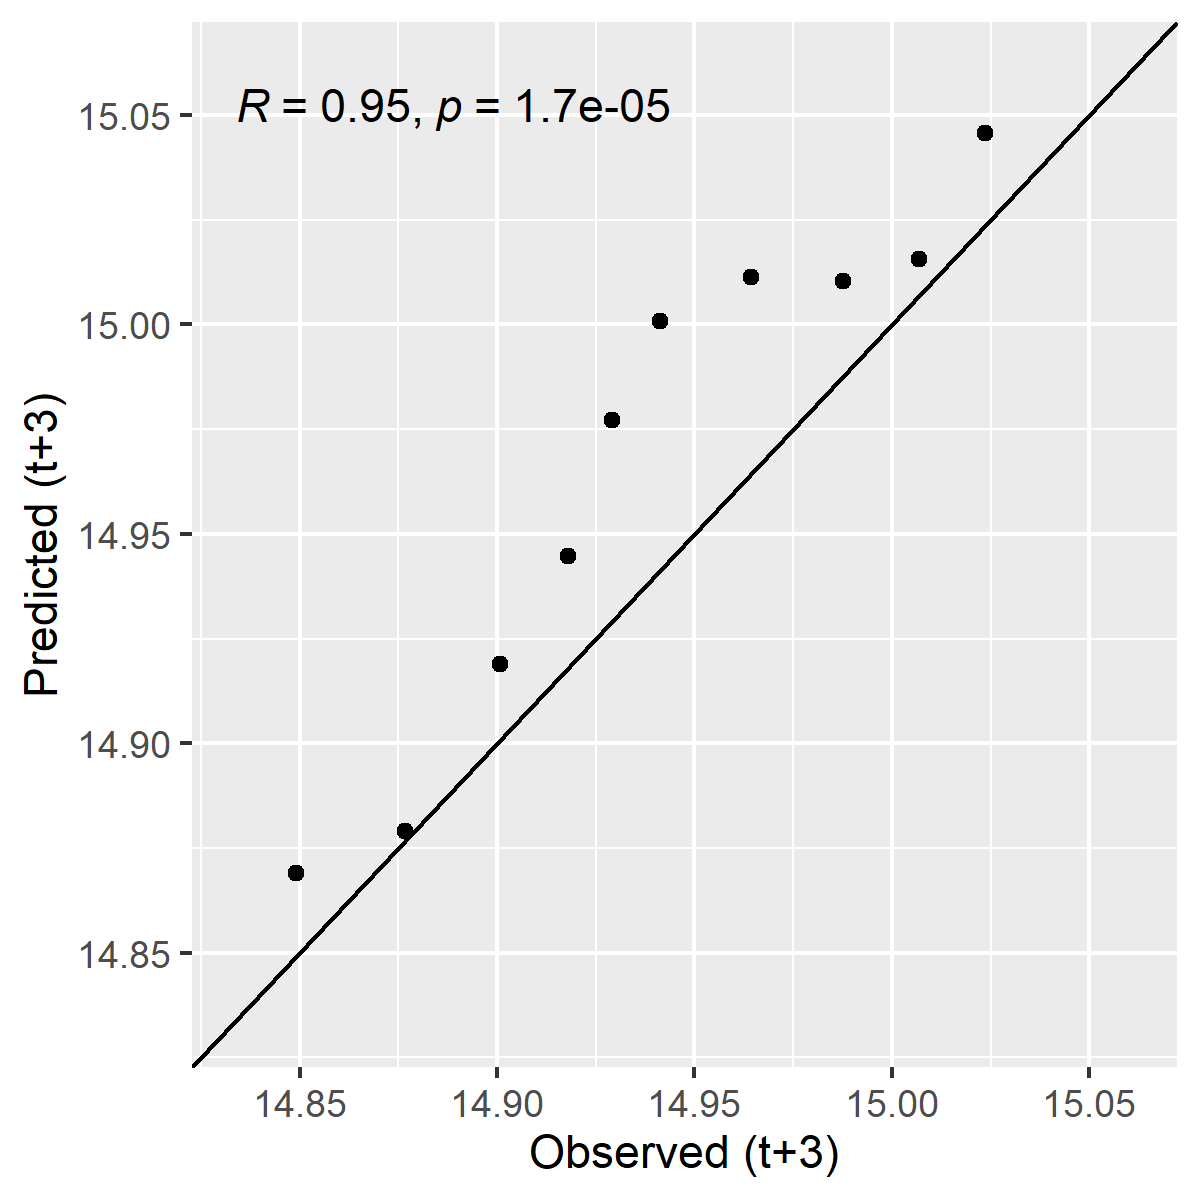
\includegraphics[width=0.3\linewidth]{day3} 
				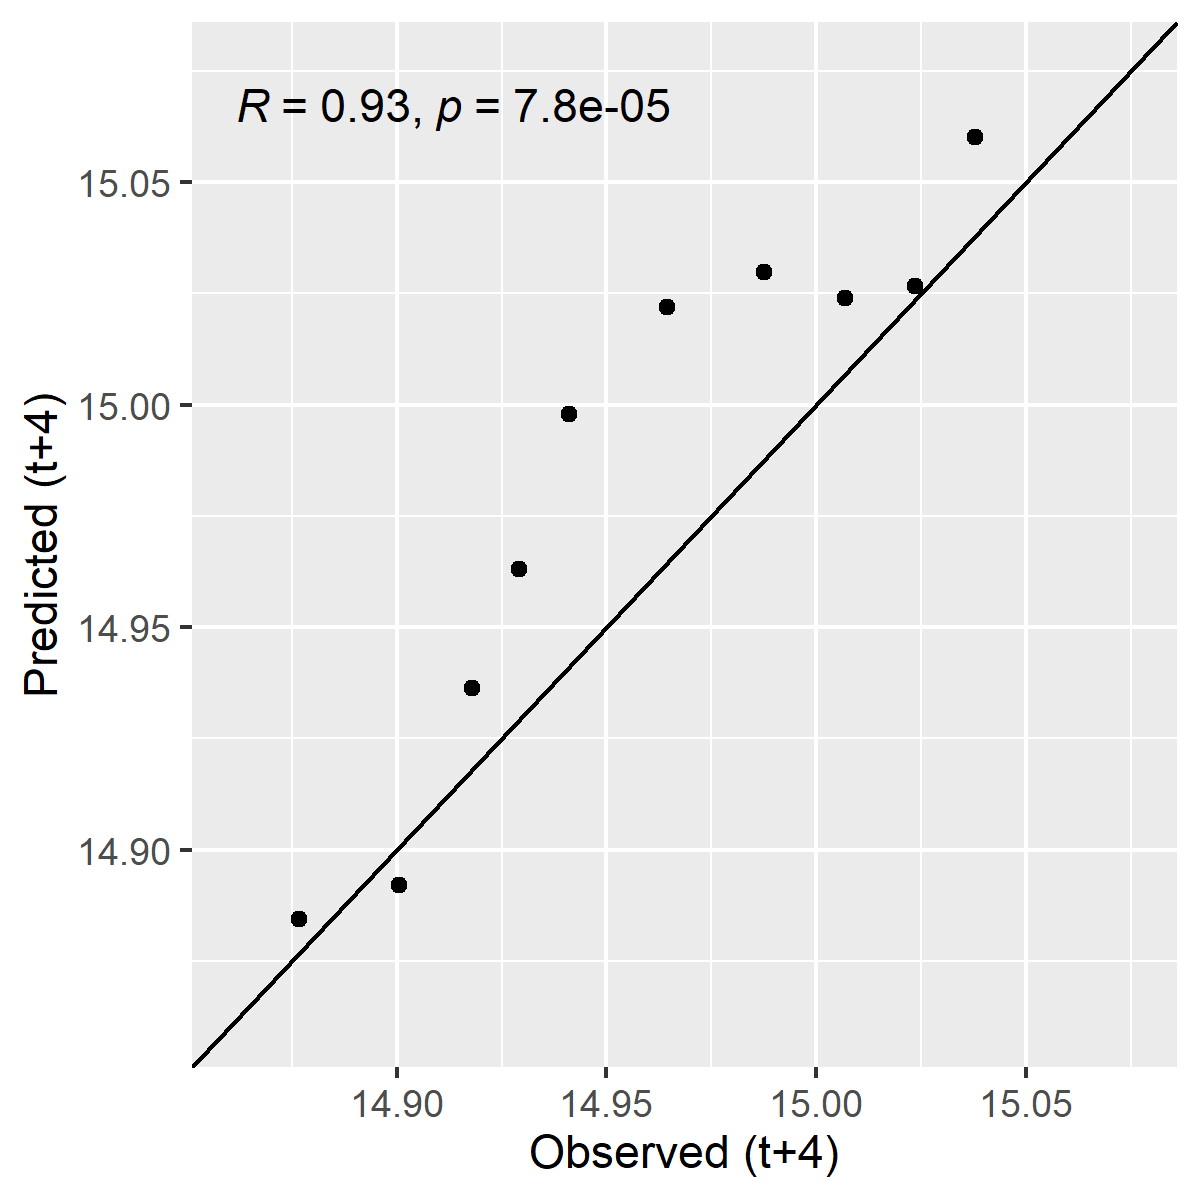
\includegraphics[width=0.3\linewidth]{day4} 
					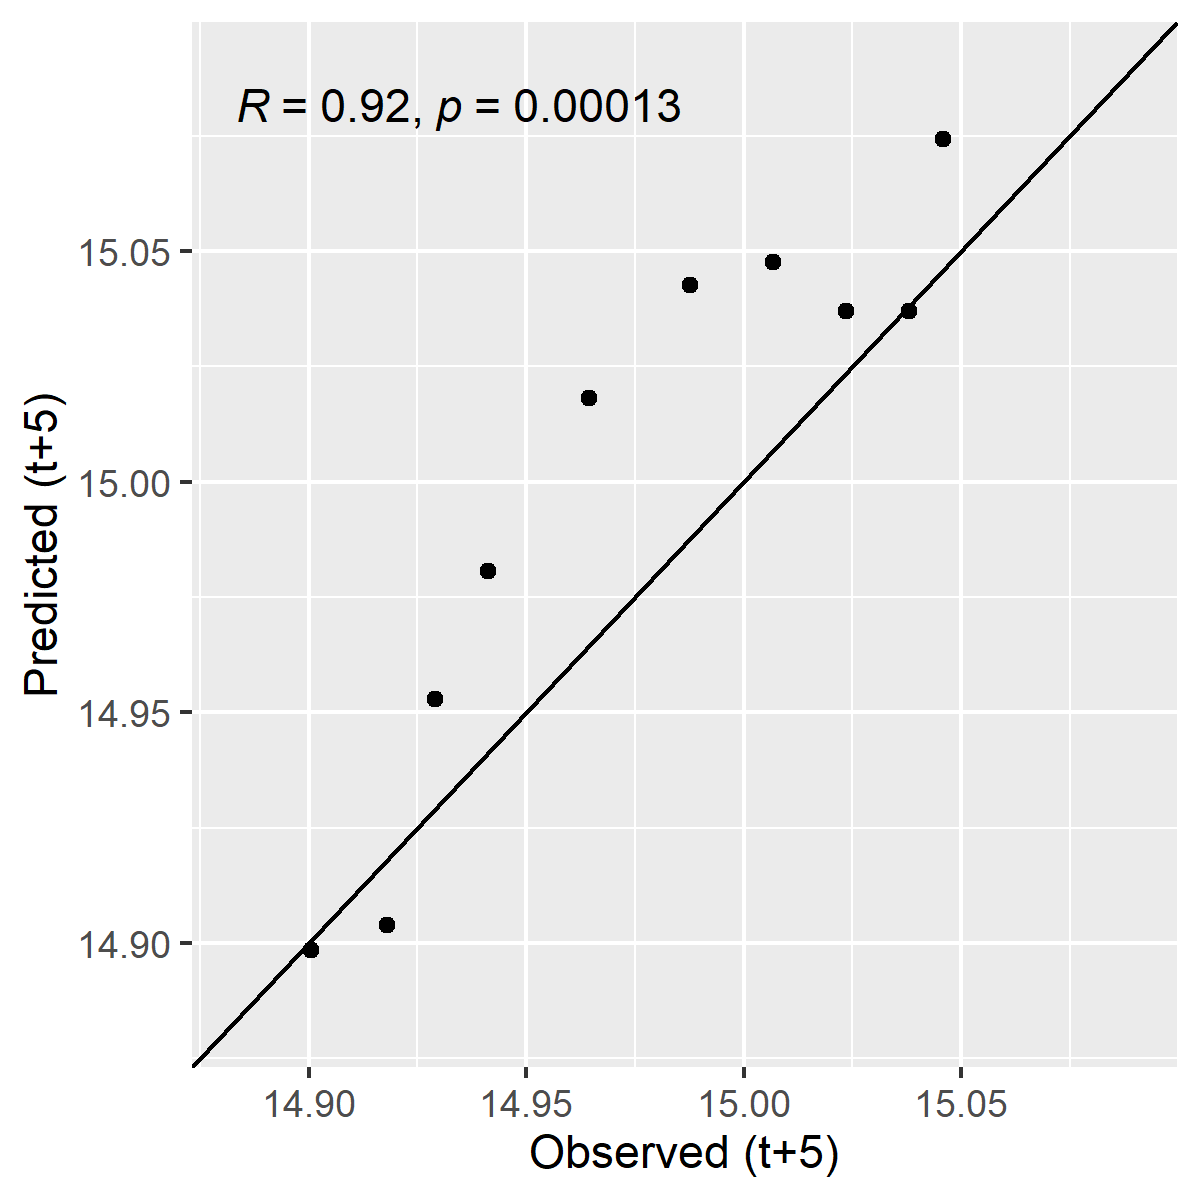
\includegraphics[width=0.3\linewidth]{day5} 
						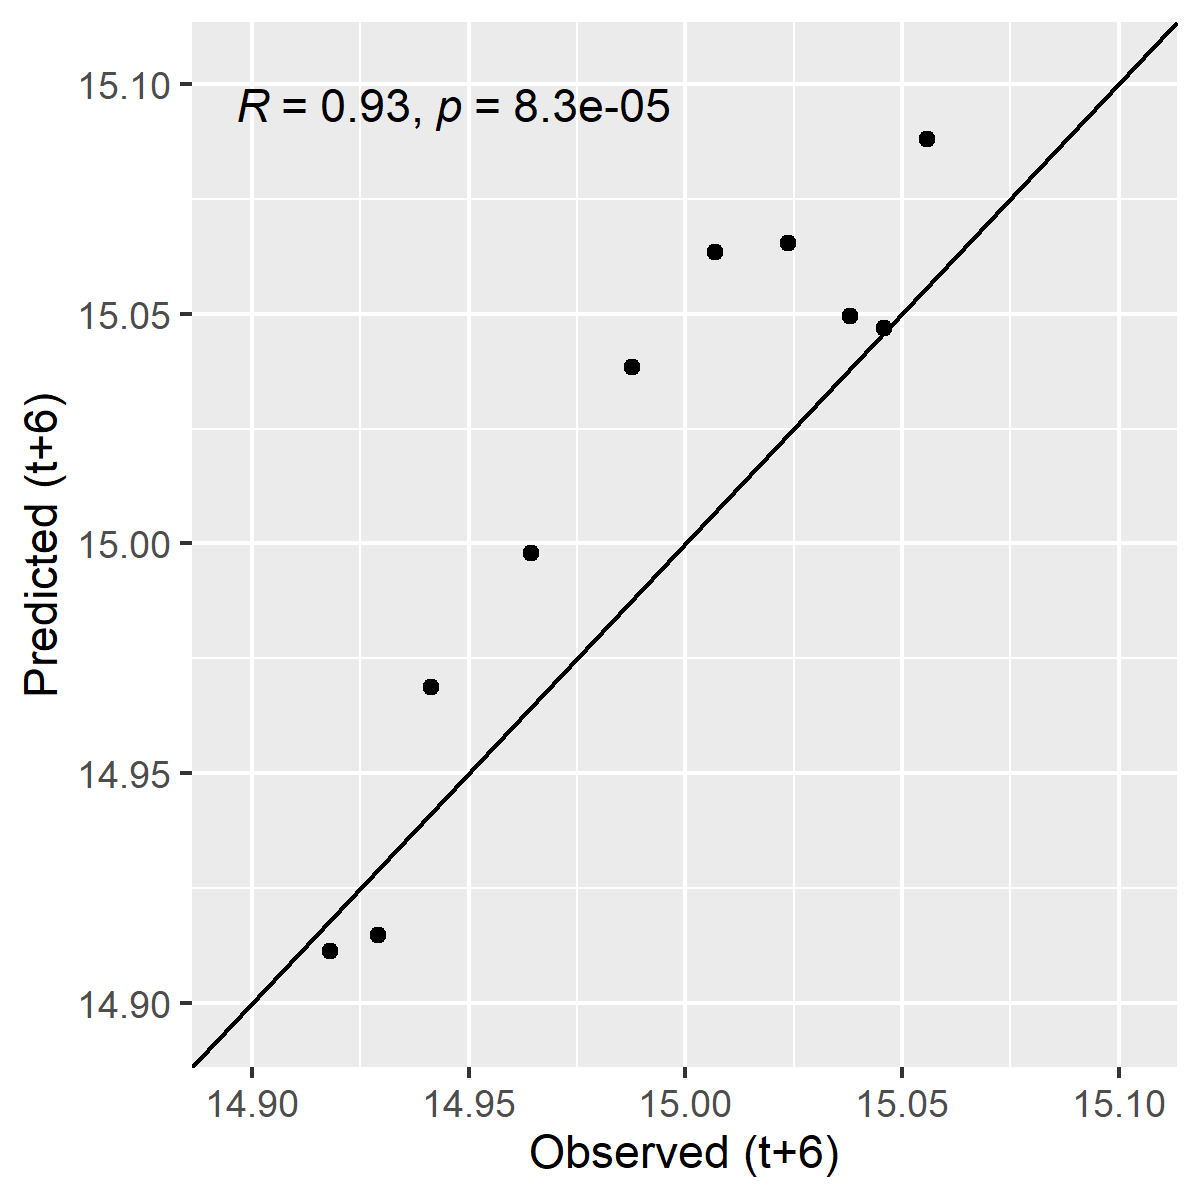
\includegraphics[width=0.3\linewidth]{day6} 
							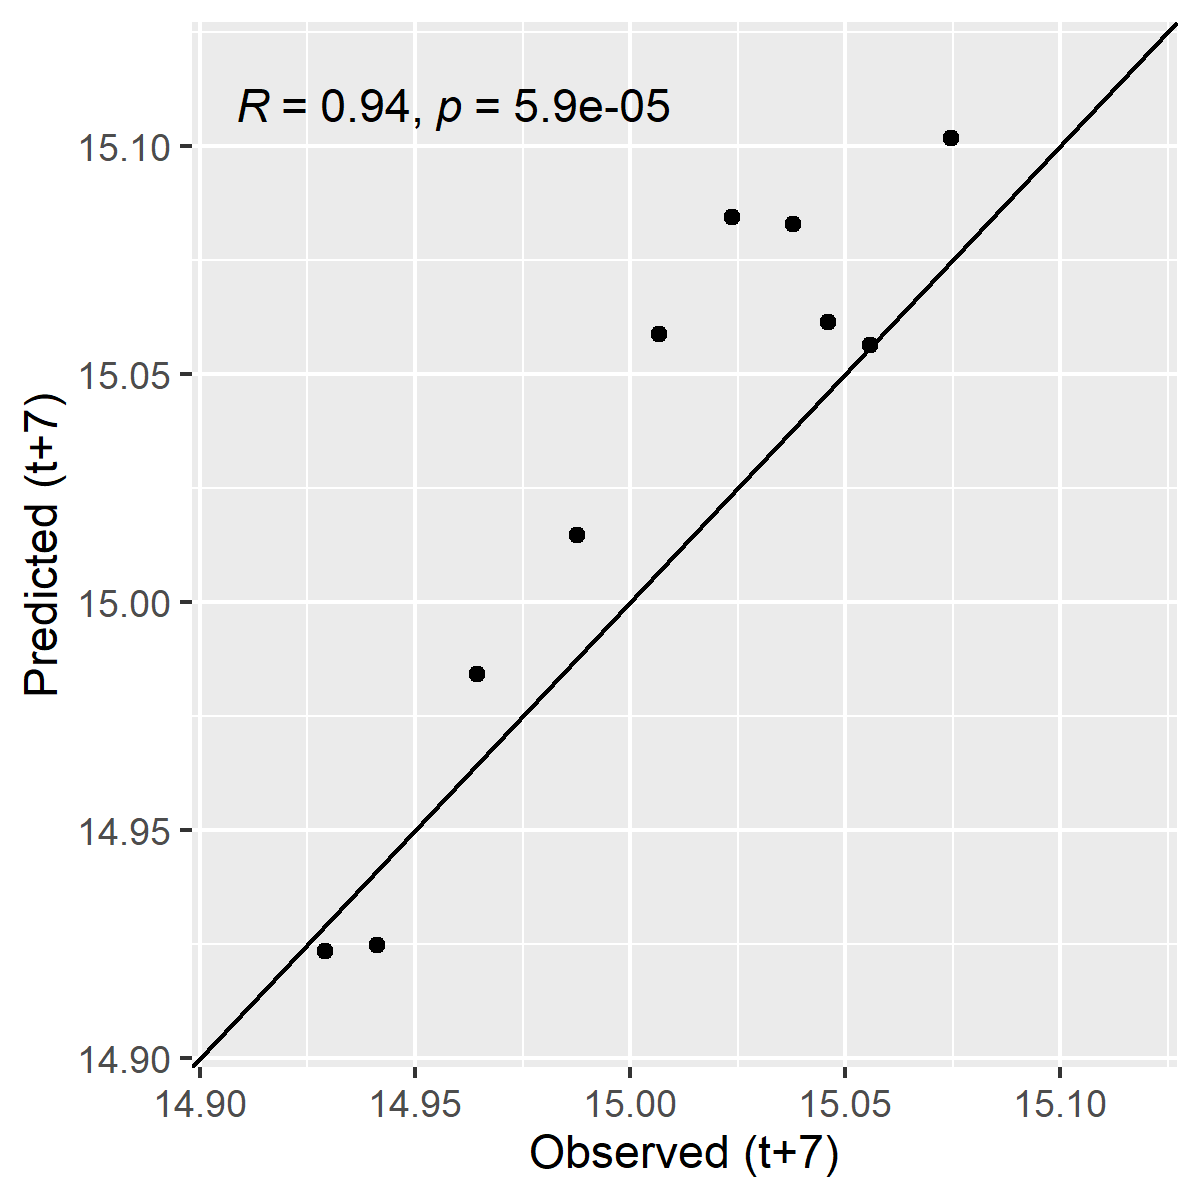
\includegraphics[width=0.3\linewidth]{day7} 
								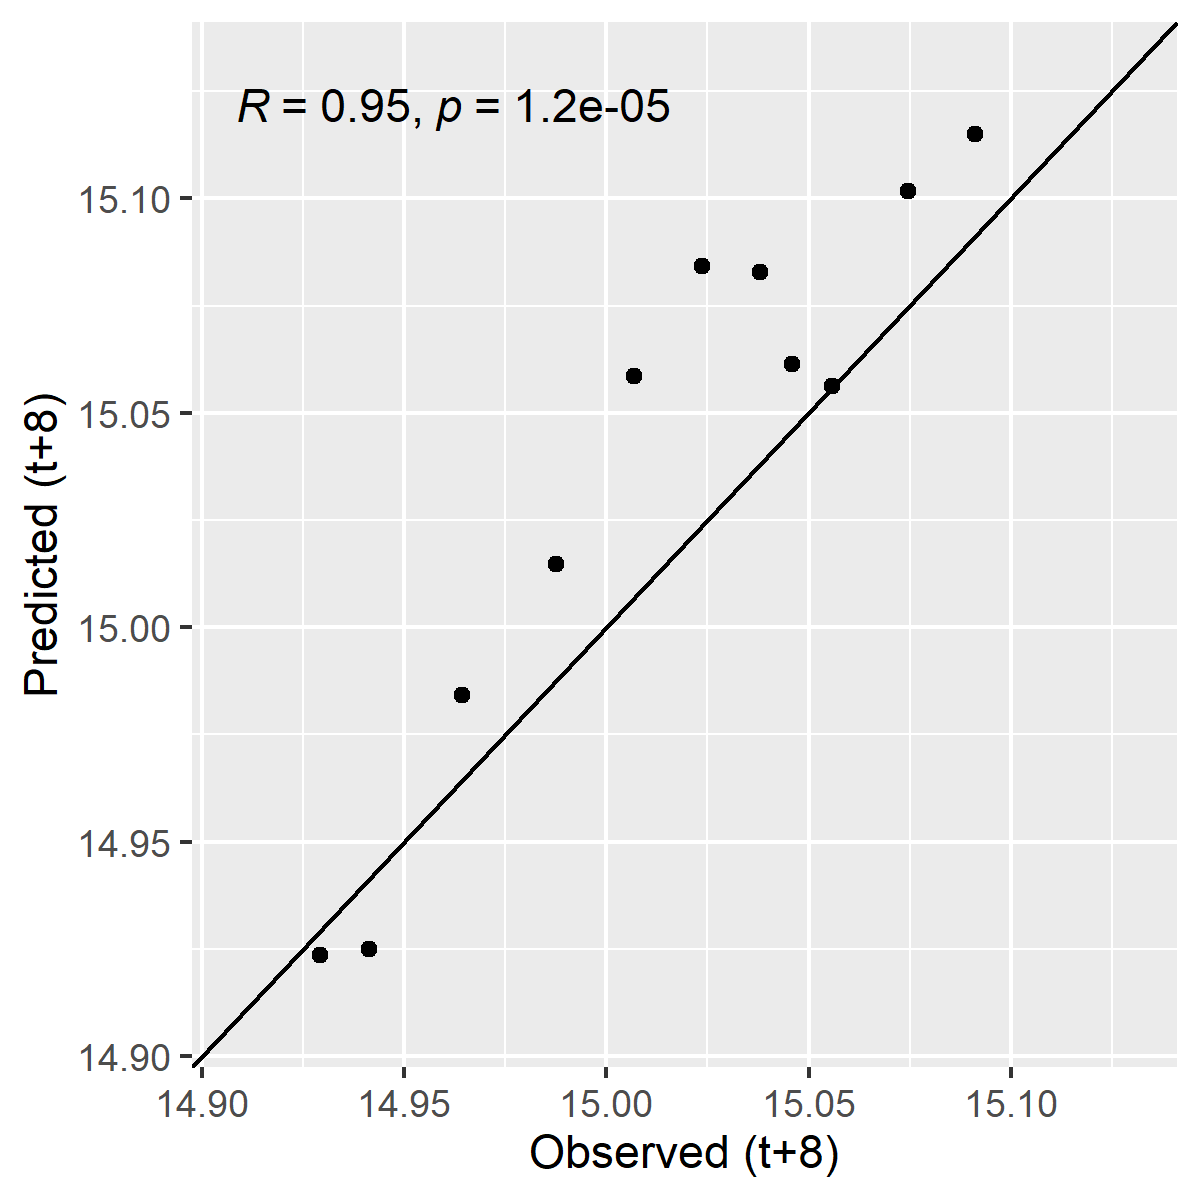
\includegraphics[width=0.3\linewidth]{day8}
									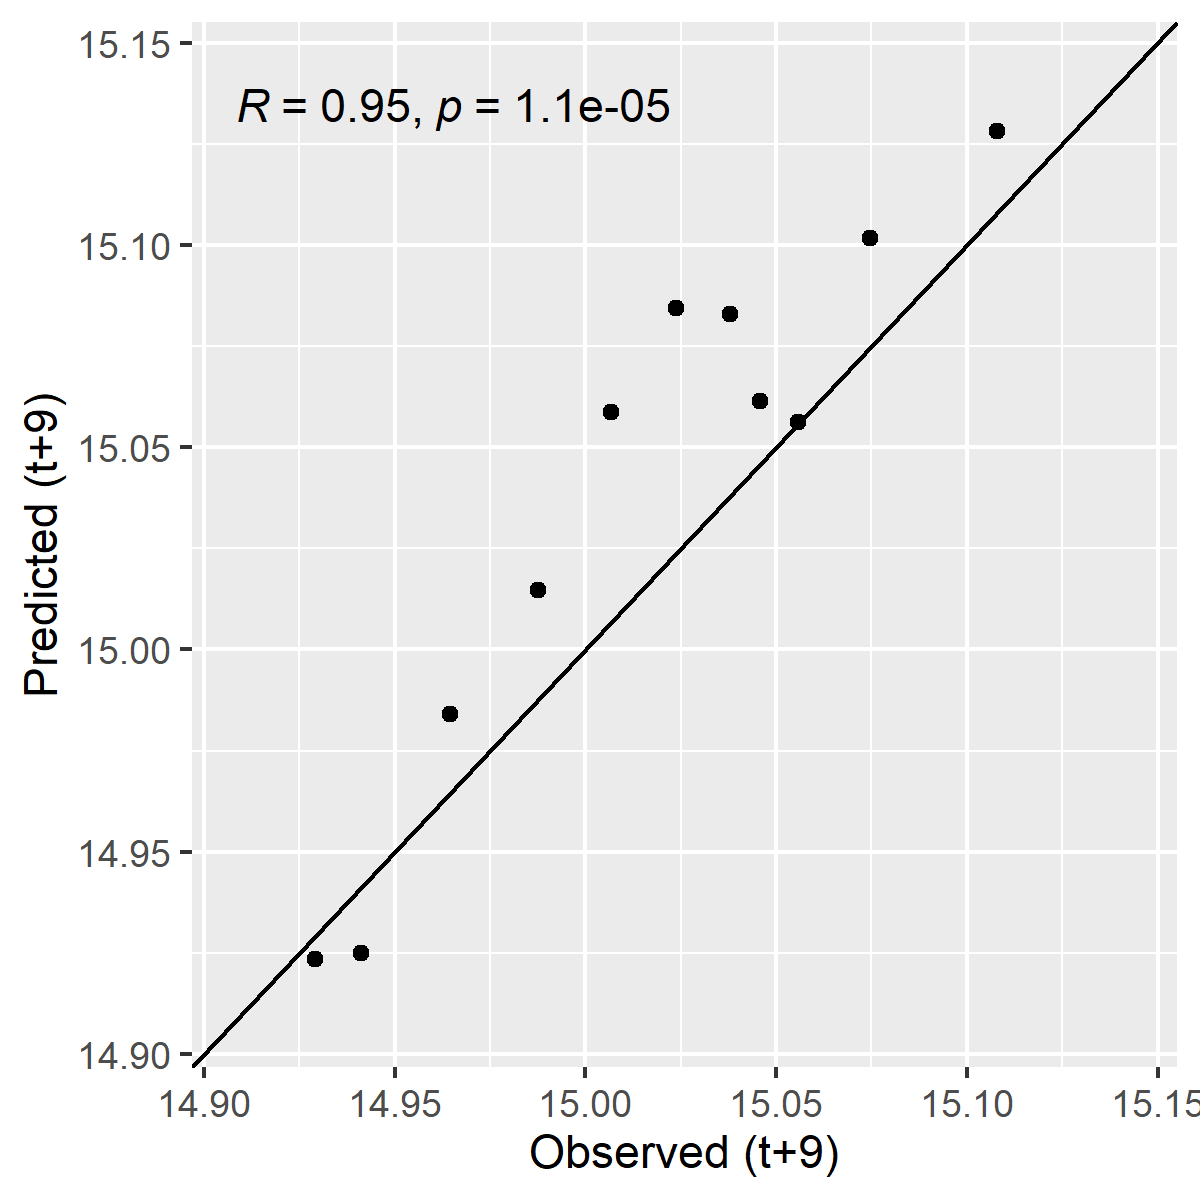
\includegraphics[width=0.3\linewidth]{day9}
										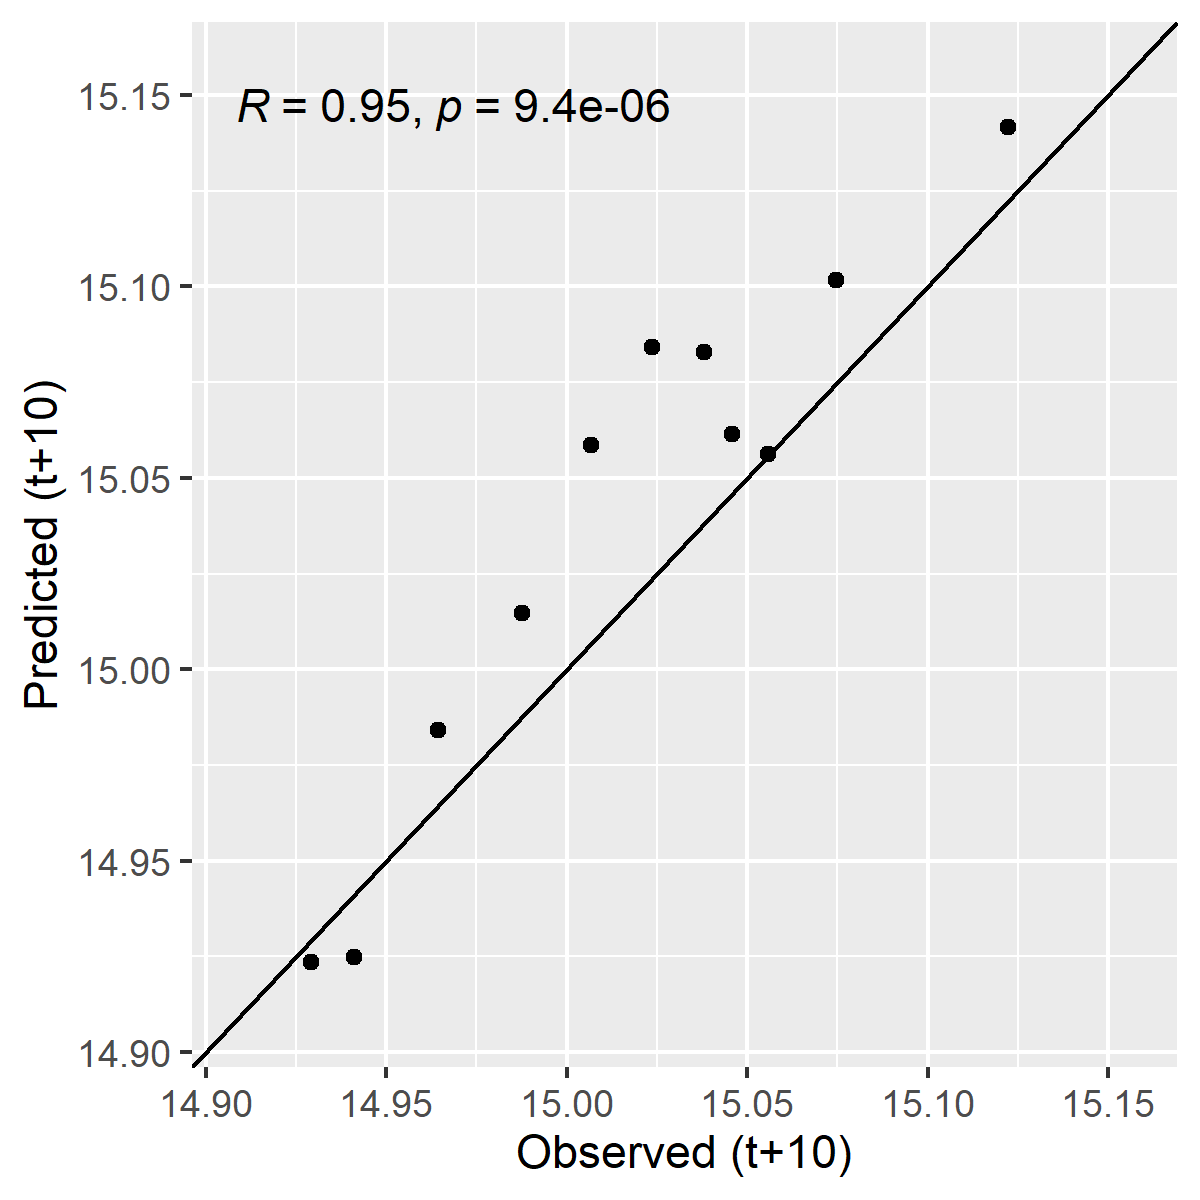
\includegraphics[width=0.3\linewidth]{day10}   
	\caption{Predicted vs observed cumulative COVID-19 cases per 100, 000 in South Africa under the RW(2) model. Base estimation period day 0 - 12/03/2020 to day t - 07/02/2021. The estimation period was expanded until 17/02/2021 one day at a time}\label{fig:accuracy2}
\end{figure}


\end{document}

